\chapter{Esame intraoperatorio: finalità e mezzi}


\section{Introduzione}
L'esame intraoperatorio ha rivoluzionato la patologia chirurgica, portando il patologo all'interno della sala operatoria. Originariamente, i chirurghi operavano solo su anomalie palpabili al seno e facevano diagnosi macroscopica (e grossolana) per differenziare tra benigno e maligno. Nella storia della medicina si riporta spesso la diagnosi di comedocarcinoma (carcinoma duttale in situ) descritto da Halsted e Bloodgood nel 1893 mediante semplice ispezione macroscopica:
\begin{quote}
    "Assistetti il Dr. Halsted nell'esplorazione di un tumore clinicamente benigno al seno. Nel momento in cui lo sezionammo, apparvero molti cilindri grigiastri e granulari dalla superficie, che chiamai allora comedoni. Sulla base dell'aspetto macroscopico del tumore, diagnosticammo la malignità e procedemmo con un intervento radicale. I linfonodi non risultavano coinvolti."
\end{quote}

\section{Veloce ma non velocissima}
Tuttavia Bloodgood riporta che alcuni anni prima (1891):
\begin{quote}
    "Il Dr. Halsted rimosse un tumore al seno che considerava clinicamente benigno. Dopo la rimozione, mentre sezionava il tumore, manifestò dubbi sulla sua natura. Chiese una diagnosi con sezione congelata inviando l’esemplare a Dr. Welch nel laboratorio patologico, a circa cinque minuti di cammino. Quando Welch raggiunse la sala operatoria, Halsted aveva già concluso l'operazione e chiuso la ferita. Da quel momento, Halsted non chiese più una seconda sezione congelata in sala operatoria per oltre venticinque anni."
\end{quote}

\section{La Richiesta di Consulenze in Sala Operatoria}
Già nel 1905, il chirurgo William J. Mayo espresse l'importanza di poter avere una diagnosi istopatologica in tempo reale durante l'intervento:
\begin{quote}
    "Vorrei che voi patologi trovaste un modo per dirci se una crescita è cancro o meno mentre il paziente è ancora sul tavolo operatorio."
\end{quote}
\textbf{Louis Blanchard Wilson} (1866–1943) sviluppò il primo metodo rapido per preparare tessuti per il microscopio (Figura \ref{fig:wilson}) e rispondendo alle esigenze dei colleghi chirurghi: ``l'intero processo può essere completato in un minuto e mezzo.''

\begin{figure}[p]
    \centering
    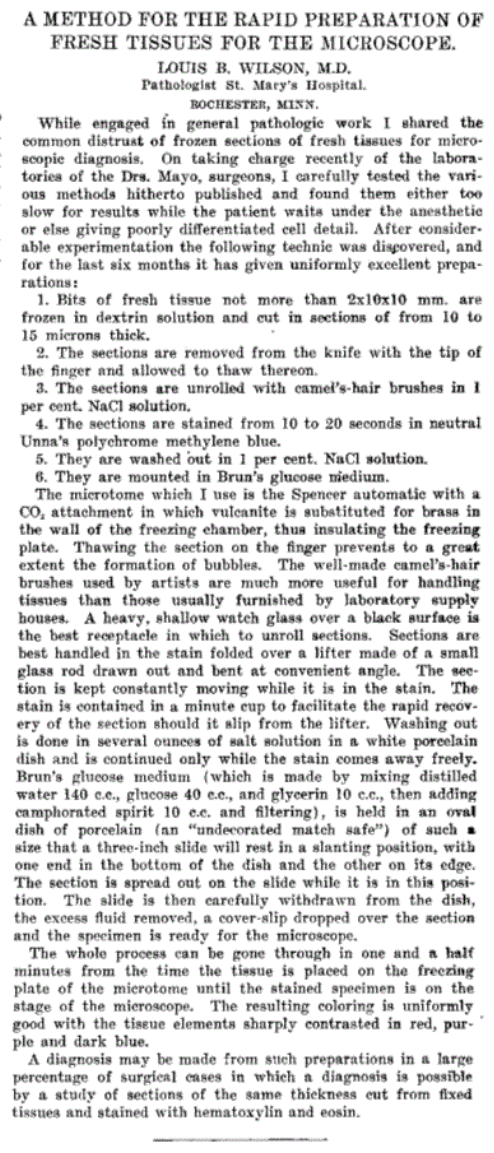
\includegraphics[width=0.5\textwidth]{Wilson1905}
    \caption{Wilson, L. B. A method for the rapid preparation of tissues for the microscope. J. Am. Med. Assoc. 45, 1737 (1905).
}
    \label{fig:wilson}
\end{figure}

\section{Glossario}
Esistono diversi termini per descrivere l'esame intraoperatioro:
\begin{itemize}
    \item Esame microscopico di tessuto fresco congelato
    \item Diagnosi su tessuto fresco
    \item Sezione rapida
    \item Sezionamento criogenico
    \item Sezione congelata
    \item Diagnosi patologica intraoperatoria
    \item Consulto intraoperatorio
    \item Esame intraoperatorio con sezione congelata (\emph{frozen section examination }FSE)
\end{itemize}
Tutti questi termini sottolineano l'aspetto procedurale del congelamento. La diagnosi intraoperatoria, analogamente alla diagnosi su sezioni stabili, si può comporre anche della parte macroscopica e per alcune patologie la valutazione macroscopica dei margini è l'unica richiesta.

\section{Finalità del FSE}
Il principale obiettivo dell'Esame con Sezione Congelata (FSE) è fornire una valutazione istologica rapida che permetta decisioni terapeutiche in tempo reale, essenziali nelle procedure intra- o peri-operatorie. Questo strumento diagnostico è cruciale in situazioni in cui la conferma immediata della natura patologica del tessuto influenza direttamente il corso dell’intervento e, in ultima analisi, l'outcome del paziente. 

Le diagnosi per le quali l'FSE è comunemente richiesto includono:
\begin{itemize}
    \item \textbf{Identificazione di processi patologici sconosciuti:} In presenza di tessuti o lesioni la cui natura non è chiara, l'FSE permette di determinare se il processo è maligno, benigno o reattivo, consentendo di adattare la procedura chirurgica alle necessità del paziente.
    \item \textbf{Valutazione dei margini di resezione:} Uno degli usi più frequenti dell'FSE è la verifica dei margini chirurgici per garantire che tutto il tessuto neoplastico sia stato rimosso, riducendo il rischio di recidiva e minimizzando la necessità di interventi aggiuntivi.
    \item \textbf{Identificazione di metastasi nei linfonodi:} L'FSE permette di rilevare la presenza di metastasi linfonodali, informazione essenziale in neoplasie come il carcinoma mammario o il melanoma, dove il coinvolgimento linfonodale può influenzare il piano di trattamento post-operatorio.
    \item \textbf{Conferma della presenza di tessuto lesionale:} Prima della rimozione definitiva o della raccolta di campioni per studi speciali, l'FSE conferma che il tessuto lesionale è presente, riducendo l'invasività della procedura e ottimizzando il campionamento per l'analisi finale.
\end{itemize}

\section{Limiti delle Sezioni Congelate}
Le sezioni congelate rappresentano uno strumento essenziale nella diagnostica intraoperatoria, ma presentano alcuni limiti significativi rispetto alle sezioni permanenti. Questi limiti devono essere ben compresi da patologi e chirurghi per evitare interpretazioni errate o decisioni operative subottimali.

\begin{itemize}
    \item \textbf{Campionamento:} A causa della necessità di operare rapidamente, il tessuto disponibile per l'FSE può essere ridotto, il che comporta un rischio di rappresentazione incompleta. Questo aspetto è particolarmente rilevante nei casi di valutazione dei margini chirurgici dove i margini possono risultare difficili da interpretare.
    \item \textbf{Assenza di studi speciali:} Le sezioni congelate non consentono l'esecuzione di colorazioni speciali, immunoistochimica o altre tecniche avanzate, che spesso sono fondamentali per una diagnosi definitiva. L'assenza di questi studi riduce la capacità diagnostica dell'FSE, specialmente per patologie rare o complesse.
    \item \textbf{Artefatti di congelamento e colorazione:} Il processo di congelamento rapido e colorazione affrettata può introdurre artefatti che complicano l'interpretazione microscopica. Ad esempio, le distorsioni cellulari indotte dal congelamento possono mascherare i dettagli morfologici e interferire con l’accuratezza della diagnosi.
\end{itemize}

\section{Artefatti}
Gli artefatti derivanti dal processo di congelamento e dalla colorazione rapida possono influire negativamente sull’accuratezza diagnostica. Minimizzare tali artefatti è essenziale per mantenere la qualità dell'FSE e garantire diagnosi precise.

\textbf{Artefatti di Congelamento:} Questi artefatti si manifestano quando il tessuto subisce il congelamento rapido necessario per il taglio istologico. Tra gli effetti più comuni vi sono la formazione di cristalli di ghiaccio che possono dislocare le strutture cellulari e mascherare dettagli importanti. L'uso di criostati moderni e di tecniche di congelamento controllato riduce l’incidenza di questi problemi.

\textbf{Artefatti di Colorazione:} La colorazione accelerata del campione, necessaria per la diagnosi intraoperatoria, può comportare variazioni nell'intensità dei coloranti, alterando la qualità dell'immagine microscopica. L’adozione di protocolli standardizzati e la scelta di coloranti ottimali sono strategie efficaci per limitare tali artefatti.

\section{FSE Inappropriate}
L'uso dell'FSE dovrebbe essere attentamente valutato per evitare interventi non necessari o dannosi per il paziente. Si riconoscono tre principali categorie di sezioni congelate inappropriate:

\begin{enumerate}
    \item \textbf{Inappropriate, ma non dannose per il paziente:} Ad esempio, eseguire una sezione congelata su una massa tumorale ampia senza che sia previsto ulteriore trattamento chirurgico fino alla diagnosi definitiva può rappresentare un uso inefficiente delle risorse, aumentando i costi della procedura senza apportare benefici clinici.
    
    \item \textbf{Inappropriate e potenzialmente dannose:} In casi di lesioni primarie molto piccole, come alcune lesioni cutanee pigmentate o noduli al seno, l’intero tessuto potrebbe essere compromesso. Le lesioni pigmentate, in particolare, sono soggette a distorsione durante il congelamento, rendendo difficile una diagnosi accurata e potenzialmente impedendo l’analisi permanente.
    
    \item \textbf{Bassa sensibilità e specificità, ma raramente utili:} In alcune situazioni particolari, come l’esame dei margini di lesioni follicolari tiroidee, il FSE potrebbe risultare d’aiuto in casi specifici, ma con sensibilità e specificità limitate. È essenziale che il chirurgo sia informato della possibilità di cambiamenti nella diagnosi su sezioni permanenti, e in questi casi è cruciale una collaborazione stretta con il patologo.
\end{enumerate}

\section{Consulto Intraoperatorio}
Il consulto intraoperatorio con il patologo prima dell'FSE è un elemento essenziale per assicurare un’interpretazione accurata e appropriata del tessuto. Ecco alcuni elementi da considerare:

\begin{itemize}
    \item \textbf{Identificatori del paziente e storia clinica rilevante:} Il chirurgo dovrebbe fornire informazioni dettagliate sul paziente e sulle patologie in corso, soprattutto in presenza di infezioni come HIV, epatite B o C, e tubercolosi (TB), che rappresentano un rischio per il personale di laboratorio.
    \item \textbf{Conferma delle caratteristiche del campione:} Un’accurata documentazione delle caratteristiche macroscopiche del campione e la conferma della sua posizione anatomica sono indispensabili. Questa documentazione fornisce una base per confronti futuri, facilitando l'interpretazione dei risultati.
    \item \textbf{Motivo dell'esame intraoperatorio:} Se lo scopo dell'esame intraoperatorio non è chiaro, bisogna contattare il chirurgo per evitare azioni inappropriate.
\end{itemize}

\section{Accuratezza della Sezione Congelata}
L'accuratezza dell'FSE varia in base all'obiettivo diagnostico specifico. Per quanto riguarda la valutazione dei margini, le metastasi linfonodali e l’identificazione tissutale, l'accuratezza può raggiungere il 100\%. Tuttavia, per la diagnosi di processi patologici sconosciuti, l'accuratezza è inferiore, approssimativamente all'80\%.

In generale, l'FSE ha un’accuratezza riportata tra il 94\% e il 97\% rispetto alla sezione permanente. Il College of American Pathologists (CAP) suggerisce che un tasso accettabile di discrepanza significativa sia intorno al 3\%, un valore considerato sicuro per l'accuratezza diagnostica in ambito intraoperatorio.

\section{Conclusioni}
L'uso dell'FSE deve essere riservato a situazioni in cui è probabile che il risultato influenzi la gestione intra- o peri-operatoria del paziente. Sebbene l'FSE offra alta accuratezza in molte applicazioni, è necessario che chirurghi e patologi siano consapevoli dei suoi limiti, lavorando insieme per garantire la sicurezza e l’efficacia delle decisioni cliniche. Il ruolo del patologo è quindi quello di mediare tra le esigenze diagnostiche e la sicurezza del paziente, evitando sezioni congelate inutili o inappropriate.
